\documentclass{beamer}
%**************************************************************
% Packages
%**************************************************************
\usepackage[utf8]{inputenc}
\usepackage[T1]{fontenc}

\usepackage{makeidx}
\makeindex
\newenvironment{theindex}
{\let\item\par
	%definitions for subitem etc
}{}
\newcommand\indexspace{}

\usepackage{multicol}
\usepackage[english]{babel}
\usepackage{graphicx}
\usepackage[toc, acronym]{glossaries}
\usepackage[nottoc]{tocbibind}
\usepackage{transparent}
\usepackage{hyperref}
\usepackage{color}
\usepackage{epstopdf}
\usepackage{subcaption}
\usepackage{wrapfig}
\usepackage{tikz}
\usepackage{tikz-uml}
\usetikzlibrary{calc,trees,positioning,arrows,chains,shapes.geometric,decorations.pathreplacing,decorations.pathmorphing,shapes,matrix,shapes.symbols}
\usepackage{setspace}
\usepackage{appendixnumberbeamer}

%**************************************************************
% Setup
%**************************************************************

% Line spaceing
\renewcommand{\baselinestretch}{1.5}

% Links color
\hypersetup {
	colorlinks=true,
	linkcolor=black,
	urlcolor=blue,
	citecolor=black
}

% Diagrams
\tikzset{
	>=stealth',
	punktchain/.style={
		rectangle, 
		rounded corners, 
		fill=yellow!20,
		draw=black, very thick,
		text width=10em, 
		minimum height=3em, 
		text centered, 
		on chain},
	line/.style={draw, thick, <-},
	element/.style={
		tape,
		top color=white,
		bottom color=blue!50!black!60!,
		minimum width=8em,
		draw=blue!40!black!90, very thick,
		text width=10em, 
		minimum height=3.5em, 
		text centered, 
		on chain},
	every join/.style={->, thick,shorten >=1pt},
	decoration={brace},
	tuborg/.style={decorate},
	tubnode/.style={midway, right=2pt},
}

\makeglossary
%\makenoidxglossaries
%**************************************************************
% Glossary definition
%**************************************************************
\newglossaryentry{package} {
	name=package,
	description={ in informatica è, un raggruppamento di classi, metodi programmi, librerie e procedure che sono logicamente collegate tra di loro
	},
	plural=packages
}
\newglossaryentry{task} {
	name=task,
	description={ è un compito secondo la definizione dello standard ISO/IEC 12207
	},
	plural=tasks
}
\newglossaryentry{Gantt} {
	name=Gantt,
	description={  è un diagramma di supporto alla gestione dei progetti
	}
}
\newglossaryentry{custom} {
	name=custom,
	description={ è un attributo con cui si indica un manufatto, un dispositivo, o un componente, progettato e realizzato su misura in base alle necessità dell'acquirente o della funzione specifica che è destinato ad assolvere
	}
}
\newglossaryentry{APIg} {
	name={API},
	description={ è l'acronimo per Application Programming Interface (in italiano interfaccia di programmazione di un'applicazione), in informatica, indica ogni insieme di procedure disponibili al programmatore, di solito raggruppate a formare un set di strumenti specifici per l'espletamento di un determinato compito all'interno di un certo programma. Spesso con tale termine si intendono le librerie software disponibili in un certo linguaggio di programmazione
	}
}

\newglossaryentry{provider} {
	name=provider,
	description={ è un'espressione inglese che indica imprese che forniscono servizi di vario tipo,  italiano si è soliti tradurre "service provider" letteralmente, chiamando l'impresa "fornitore di servizi"
	},
	plural=providers
}
\newglossaryentry{token} {
	name=token,
	description={ con questo termine si fa riferimento ai Json Web Token (o JWT) che sono stringhe di caratteri alfanumerici che tipicamente incapsulano le credenziali di sicurezza per una sessione di login, identificando l'utente della stessa. Questi token sono segnati da una chiave del server grazie la quale è possibile verificarne la veridicità
	}
}
\newglossaryentry{header} {
	name=header,
	description={ o intestazione, è una parte del pacchetto ,inviato nelle richieste http, che contiene le informazioni di controllo necessarie al funzionamento della rete cioè le informazioni di protocollo aggiunte di strato in strato
	},
	plural=headers
}
\newglossaryentry{endpoint} {
	name=endpoint,
	description={ è l'url attraverso il quale un'applicazione client può accedere ad un servizio web. Lo stesso servizio web di solito ha endpoint multipli
	},
	plural=endpoints
}
\newglossaryentry{JSONg} {
	name={JSON},
	description={  acronimo di Javascript Object Notation, è un formato adatto all'interscambio di dati fra applicazioni client-server
	}
}

\newglossaryentry{REST-based} {
	name=REST-based,
	description={ fa riferimento ad architetture o chiamate  basate sul protocollo REST (vedi sez. \ref{rest})
	}
}
\newglossaryentry{JOIN} {
	name=JOIN,
	description={  è una clausola del linguaggio SQL che serve a combinare (unire) le tuple di due o più relazioni di un database tramite l'operazione di congiunzione (od unione) dell'algebra relazionale
	}
}
\newglossaryentry{SQL} {
	name=SQL,
	description={ è un linguaggio standardizzato per database basati sul modello relazionale
	}
}
\newglossaryentry{query} {
	name=query,
	description={ indica l'interrogazione da parte di un utente di un database, strutturato tipicamente secondo il modello relazionale, per compiere determinate operazioni sui dati
	},
	plural=queries
}
\newglossaryentry{framework} {
	name=framework,
	description={  architettura o struttura di supporto su cui un programma può essere creato. In genere è composto da una serie di librerie e strumenti di sviluppo
	},
	plural=frameworks
}
\newglossaryentry{virtual machine} {
	name=virtual machine,
	description={ o macchina virtuale (VM), viene indicato un software che, attraverso un processo di virtualizzazione, crea un ambiente virtuale che emula tipicamente il comportamento di una macchina fisica grazie all'assegnazione di risorse hardware
	},
	plural=virtual machines
}
\newglossaryentry{Design Pattern} {
	name=Design Pattern,
	description={ nell'ambito dell'ingegneria del software, un design pattern, è un concetto che può essere definito "una soluzione progettuale generale ad un problema ricorrente". Si tratta di una descrizione o modello logico da applicare per la risoluzione di un problema che può presentarsi in diverse situazioni durante le fasi di progettazione e sviluppo del software, ancor prima della definizione dell'algoritmo risolutivo della parte computazionale
	},
	plural=Design Patterns
}
\newglossaryentry{stateless} {
	name=stateless,
	description={ è un protocollo di comunicazione che tratta ogni richiesta come una transazione indipendente, scollegata da qualsiasi precedente richiesta, rendendo la comunicazione composta da coppie indipendenti di richiesta e risposta. Un protocollo stateless inoltre non richiede che il server mantenga le informazioni della sessione per ogni partner di comunicazione per la durata di multiple richieste
	}
}
\newglossaryentry{caching} {
	name=caching,
	description={ è il processo di immagazzinamento dati in una cache, che è una memoria temporanea
	}
}
\newglossaryentry{UML} {
	name=UML,
	description={ è un linguaggio di modellazione e specifica basato sul paradigma object-oriented
	}
}
\newglossaryentry{route} {
	name=route,
	description={ ci si riferisce alla definizione di un URI e a come esso risponde ad una specifica richiesta HTTP di un client
	},
	plural=routes
}
\newglossaryentry{generic} {
	name=generic,
	description={ è un tipo di dato utilizzato negli algoritmi di programmazione che non ha la necessità di essere istanziato immediatamente, bensì può essere specificato in un secondo momento
	},
	plural=generics
}
\newglossaryentry{accessor} {
	name=accessor,
	description={per il linguaggio di programmazione C\# un accessor di una proprietà (o campo dati di una classe) contiene il codice associato con l'operazione di \textit{getting} (lettura) o il \textit{setting} (scrittura) della proprietà stessa. La dichiarazione un un accessor può contenerne uno di tipo \textit{get}, uno di tipo \textit{set} o entrambi
	},
	plural=accessors
}
\newglossaryentry{getter} {
	name=getter,
	description={ è un metodo di una classe utilizzato per leggere il valore di un campo dati della stessa
	},
	plural=getters
}
\newglossaryentry{setter} {
	name=setter,
	description={ è un metodo di una classe utilizzato per scrivere il valore di un campo dati della stessa
	},
	plural=setters
}

\newglossaryentry{URLg} {
	name={URL},
	description={ o Uniform Resource Locator è una sequenza di caratteri che identifica univocamente l'indirizzo di una risorsa in Internet, tipicamente presente su un host server
	}
}
\newglossaryentry{Debugger} {
	name=Debugger,
	description={ è un programma/software specificatamente progettato per l'analisi e l'eliminazione dei bug (debugging), ovvero errori di programmazione interni al codice di altri programmi. E' spesso compreso all'interno di un ambiente integrato di sviluppo (IDE)
	},
	plural=Debuggers
}
\newglossaryentry{logging} {
	name=logging,
	description={ è la registrazione sequenziale e cronologica delle operazioni effettuate, da un utente, un amministratore o automatizzate, man mano che vengono eseguite dal sistema o applicazione
	}
}

\newglossaryentry{asset} {
	name=asset,
	description={ è una risorsa di un azienda
	}
}


\newglossaryentry{URIg} {
	name={URI},
	description={ o Uniform Resource Identifier, in informatica, si riferisce a una stringa che identifica univocamente una risorsa generica che può essere un indirizzo Web, un documento, un'immagine, un file, un servizio, un indirizzo di posta elettronica, ecc
	}
}

\newglossaryentry{cloud-based} {
	name=cloud-based,
	description={ si indica un paradigma basato, sul Cloud, di erogazione di risorse informatiche, come l'archiviazione, l'elaborazione o la trasmissione di dati, caratterizzato dalla disponibilità on-demand attraverso Internet a partire da un insieme di risorse preesistenti e configurabili
	}
}

%**************************************************************
% Acronyms definitions
%**************************************************************
\newacronym{CRM}{CRM}{Customer relationship management}

%\newacronym{JSON}{JSON}{JavaScript Object Notation}

\newacronym{http}{HTTP}{Hypertext Transfer Protocol}

\newacronym{DAO}{DAO}{Data Access Object}

\newacronym{DTO}{DTO}{Data Transfer Object}

%\newacronym{URI}{URI}{Uniform Resource Identifier}





%%% define the acronym and use the see= option
\newglossaryentry{URI}{type=\acronymtype, name={URI}, description={Uniform Resource Identifier}, first={Uniform Resource Identifier (URI)\glsadd{URIg}}, see=[Glossary:]{URIg}}

\newglossaryentry{JSON}{type=\acronymtype, name={JSON}, description={JavaScript Object Notation}, first={JavaScript Object Notation (JSON)\glsadd{JSONg}}, see=[Glossary:]{JSONg}}

\newglossaryentry{API}{type=\acronymtype, name={API}, description={Application Programming Interface}, first={Application Programming Interface (API)\glsadd{APIg}}, see=[Glossary:]{APIg}}

\newglossaryentry{URL}{type=\acronymtype, name={URL}, description={Uniform Resource Locator}, first={Uniform Resource Locator (URL)\glsadd{URLg}}, see=[Glossary:]{URLg}}
\usetheme{Padova}

\title{Botnet Finder Framework}
\subtitle{a modular framework for botnet detectors evaluation and a practical application}
\author{Nicola De Cao}
\date{14 July 2016}

\begin{document}

	\maketitle

	\begin{frame}{Outline}
		\begin{multicols}{2}
			%\tableofcontents
			\begin{itemize}
				\item Introduction
				\begin{itemize}
					\item Botnets
					\item Detectors
				\end{itemize}
				\item The Framework
				\begin{itemize}
					\item Modules
				\end{itemize}
				\item ELISA evaluation
				\begin{itemize}
					\item Implemented detectors
					\item Experiment
					\item Results
				\end{itemize}
				\item Conclusion
			\end{itemize}
		\end{multicols}
	\end{frame}

	\section{Introduction}
	
	\subsection{Botnets}
	
	\begin{frame}{What is a Botnet?}
		\begin{figure}
			\includegraphics[width=10cm]{botnet.jpg}
		\end{figure}
	\end{frame}
	
	\begin{frame}{Botnets}
		\begin{itemize}
			\item A \textbf{network of infected machines} (bots) controlled by an attacker
			\item \textbf{Command and Control (C\&C)} channel: servers and infrastructure to communicate with bots
			\item In the past - \textbf{centralized} C\&C over {IRC} and {HTTP}
			\item Today - \textbf{decentralized} P2P communication mechanisms
		\end{itemize}
	\end{frame}
	
	\subsection{Detectors}
	
	\begin{frame}{Botnet Detectors}
		Search for C\&C communication in a network.\\
		Two main approaches:
		\begin{itemize}
			\item \textbf{Active:} modify potential C\&C packets, observe reactions;
			\item \textbf{Passive:} observe the network traffic to find:
			\begin{itemize}
				\item patterns (by correlations and behavior)
				\item clusters of similar nodes
			\end{itemize}
		\end{itemize}
	\end{frame}
	
	\begin{frame}{\ }
		\Huge \textbf{The framework}
	\end{frame}
	
	\section{The framework}
	
	\begin{frame}{BFF (Botnet Finder Framework)}
		\textbf{BFF (Botnet Finder Framework)}: a modular and extensible framework to develop and evaluate botnet detectors in \textbf{Python}. It provides tools to handle with:
		\begin{itemize}
			\item building datasets from NetFlow files
			\item features extraction
			\item classification algorithms (both supervised and unsupervised)
			\item evaluation metrics (accuracy, precision, sensitivity, etc.)
			\item plotting results
		\end{itemize}
	\end{frame}
	
	\subsection{Modules}

	\begin{frame}{Modules 1/3}
		    \begin{minipage}{.5\textwidth}
				\begin{itemize}
					\item Initially a \textbf{NetFlow} file is processed and transformed into an internal representation: a \textbf{Dataset}
					\vspace{.5em}
					\item then BFF use Datasets to extract \textbf{features} using the \textbf{extract} module
				\end{itemize}
		    \end{minipage}%
			\begin{minipage}{.6\textwidth}
				\begin{figure}
					\centering
					\begin{tikzpicture}
					[start chain=going below]
					\node[punktchain, join] (nf) {NetFlow};
					\node[punktchain, join] (ds) {Dataset};
					\node[punktchain, join] (feat) {Features};
					
					\draw[tuborg, decoration={brace}] let \p1=(nf.south), \p2=(ds.north) in ($(2.5, \y1)$) -- ($(2.5, \y2)$) node[tubnode] {build};
					\draw[tuborg, decoration={brace}] let \p1=(ds.south), \p2=(feat.north) in ($(2.5, \y1)$) -- ($(2.5, \y2)$) node[tubnode] {extract};
					\end{tikzpicture}
				\end{figure}
		  \end{minipage}
	\end{frame}
		
	\begin{frame}{Modules 2/3}
		    \begin{minipage}{.5\textwidth}			
				\begin{itemize}
					\item Once features are extracted, the \textbf{predict} module performs \textbf{predictions} over the target values
					\vspace{.5em}
					\item then BFF computes evaluation \textbf{metrics} with the \textbf{evaluate} module
				\end{itemize}
		    \end{minipage}%
		    \begin{minipage}{.6\textwidth}
				\begin{figure}
					\centering
					\begin{tikzpicture}
					[start chain=going below]
					\node[punktchain, join] (feat) {Features};
					\node[punktchain, join] (pred) {Predictions};
					\node[punktchain, join] (metr) {Metrics};
					
					\draw[tuborg, decoration={brace}] let \p1=(feat.south), \p2=(pred.north) in ($(2.5, \y1)$) -- ($(2.5, \y2)$) node[tubnode] {predict};
					\draw[tuborg, decoration={brace}] let \p1=(pred.south), \p2=(metr.north) in ($(2.5, \y1)$) -- ($(2.5, \y2)$) node[tubnode] {evaluate};
					\end{tikzpicture}
				\end{figure}
		    \end{minipage}
	\end{frame}

	\begin{frame}{Modules 3/3}
		\begin{minipage}{.5\textwidth}
	    	\begin{itemize}
	    		\item Finally, the \textbf{plot} module generates \textbf{plots} from processed metrics
	    	\end{itemize}
		\end{minipage}%
		\begin{minipage}{.6\textwidth}
			\begin{figure}
				\centering
				\begin{tikzpicture}
				[start chain=going below]
				\node[punktchain, join] (metr) {Metrics};
				\node[punktchain, join] (plot) {Plots};
				
				\draw[tuborg, decoration={brace}] let \p1=(metr.south), \p2=(plot.north) in ($(2.5, \y1)$) -- ($(2.5, \y2)$) node[tubnode] {plot};
				\end{tikzpicture}
			\end{figure}
		\end{minipage}
	\end{frame}
	
	\subsection{NetFlow}
	
	\begin{frame}{NetFlow 1/2}
		\begin{longtable}[h]{c c c}
			\hline
			\textbf{Datetime} & \textbf{Duration} & \textbf{Protocol} \\ \hline \hline
			2016-06-09 07:57:18.890838 & 0.000245 & SSL \\ \hline
			2016-06-09 07:57:18.890876 & 0.000038 & TCP \\ \hline
			2016-06-09 07:57:18.893086 & 0.000848 & HTTP \\ \hline
			2016-06-09 07:57:18.893604 & 0.000039 & SSH \\ \hline
			2016-06-09 07:57:18.930443 & 0.000001 & SSL \\ \hline
			2016-06-09 07:57:18.930715 & 0.000272 & TCP \\ \hline
		\end{longtable}
	\end{frame}
	
	\begin{frame}{NetFlow 2/2}
		\begin{longtable}[h]{r r r c}
			\hline
			\textbf{Source IP} & \textbf{Destination IP} & \textbf{Length} & \textbf{Label} \\ \hline \hline
			216.58.208.99 & 210.202.121.130 & 1484 & Benign \\ \hline
			210.202.121.130 & 216.58.208.99 & 54 & Botnet \\ \hline
			167.114.216.47 & 210.202.121.159 & 847 & Benign \\ \hline
			210.202.121.185 & 147.162.22.101 & 114 & Benign \\ \hline
			216.58.208.99 & 210.202.121.130 & 1116 & Botnet \\ \hline
			210.202.121.130 & 216.58.208.99 & 54 & Benign \\ \hline
		\end{longtable}
	\end{frame}
	
	\subsection{Extract module}
	
	\begin{frame}{Extract module}
		The \textbf{extract} module builds matrices with \textbf{features} for each sample in the dataset. This will help us finding patterns into the data in order to learn a C\&C channel behavior.
		
		\begin{minipage}{.5\textwidth}
			\begin{longtable}[h]{c c c c | c}
				$x_1$ & $x_2$ & \dots & $x_n$ & $y$ \\ \hline \hline
				1.31 & 5.8 & \dots & 0.054 & 0 \\ \hline
				4.7 & 5.22 & \dots & 8.47 & 1 \\ \hline
				18.5 & 16.2 & \dots & 0.114 & 0 \\ \hline
				9.9 & 22.3 & \dots & 6.16 & 1 \\
			\end{longtable}
		\end{minipage}%
		\begin{minipage}{.5\textwidth}
			\begin{figure}
				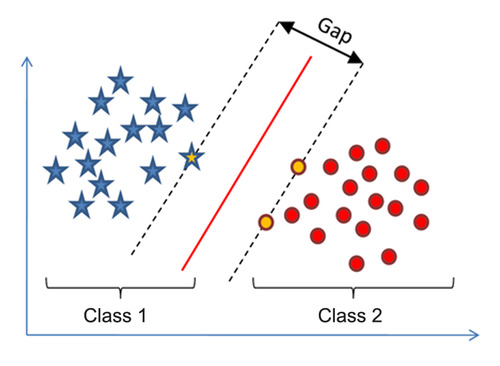
\includegraphics[width=\textwidth]{svm.jpg}
			\end{figure}
		\end{minipage}
	\end{frame}
	
	\subsection{Predict module}
	
	\begin{frame}{Predict module}
		The \textbf{predict} module trains a classifier and then performs predictions. It uses stratified k-fold to select train and test subsets properly from the original dataset.
		\begin{longtable}[h]{c c c c}
			\hline
			\textbf{Test} & \textbf{Prediction} & \textbf{Label} & \textbf{Predicted Condition } \\ \hline \hline
			0 & 0 & \textcolor{green}{Benign} & True negative \\ \hline
			0 & 1 & \textcolor{green}{Benign} & False positive \\ \hline
			1 & 1 & \textcolor{red}{Botnet} & True positive \\ \hline
			1 & 0 & \textcolor{red}{Botnet} & False negative \\ \hline
		\end{longtable}
	\end{frame}
	
	\subsection{Evaluate module}
	
	\begin{frame}{Evaluate module}
		The \textbf{evaluate} module computes the following metrics:
		
		\begin{itemize}
			\item \textbf{Accuracy:} the proportion of true results among the total number of correct or incorrect classifications
			\item \textbf{Precision:} the proportion of the samples that the classifier predicts positive and are actually positive, among all the samples that it classifies as positive
			\item \textbf{Sensitivity:} the proportion of the samples that the classifier predicts positive and are actually positive, among all the samples that are positive
		\end{itemize}

	\end{frame}
	
	\subsection{Plot module}
	
	\begin{frame}{Plot module}
		Plot module builds bar charts in order to provide a visual representation of the evaluation metrics.
	
		\begin{figure}
			\includegraphics[width=\textwidth]{BotTrack_plot_metrics_bars2.eps}
		\end{figure}
	\end{frame}
	
	\begin{frame}{\ }
		\Huge \textbf{ELISA evaluation}
	\end{frame}

	\section{ELISA evaluation}
	
	\begin{frame}{ELISA: Elusive Social Army}
		\textbf{ELISA} [1] is a botnet that propagates its command and control messages using \textbf{Facebook}. It communicates with the botmaster appending an invisible string, made of unprintable characters, on users' messages.
		
		\begin{longtable}{c c l}
			Latin Small letter A & U+0061 & $\rightarrow$ a \\
			Left-To-Right Mark & U+200E & $\rightarrow$
		\end{longtable}
		{\setstretch{1}\footnotesize
			[1] Alberto Compagno, Mauro Conti, Daniele Lain, Giulio Lovisotto, and Luigi Vincenzo Mancini. \textit{Boten ELISA: A novel approach for botnet C\&C in Online Social Networks.} In IEEE CNS 2015. \par
		}
	\end{frame}

	\subsection{Detectors}

	\begin{frame}{Detectors 1/2 - BotTrack}
		\begin{minipage}{.6\textwidth}
		\begin{itemize}
			\item \textbf{Features:} each IP is a node, flows are edges, BotTrack[2] computes hub and authority scores with \textbf{HITS}
			\item \textbf{Clustering:} uses \textbf{DBSCAN}
			\item \textbf{Classifier:} considers an IP as malicious if it is in the same cluster of a known malicious IP/node
		\end{itemize}
		\end{minipage}%
		\begin{minipage}{.45\textwidth}
			\vspace{-1cm}
			\begin{figure}
				\includegraphics[width=\textwidth]{dbscan.png}
			\end{figure}
		\end{minipage}
		
		{\setstretch{1}\footnotesize \vspace{.25cm}
			[2]	Jér\^ome François and Shaonan Wang and Radu State and Thomas Engel \emph{BotTrack: Tracking Botnets Using NetFlow and PageRank} \par
		}
	\end{frame}
	


	\begin{frame}{Detectors 2/2 - Disclosure}
		Disclosure[3] tries to find non-human patterns:
		\begin{itemize}
			\item \textbf{Features:} \textbf{flow size}-based features like statistical, autocorrelation, and unique flow size measurements; \textbf{client access patterns}-based features like regular access patterns, and unmatched flow density
			\item \textbf{Classifier:} Random Forests
		\end{itemize}
	
		{\setstretch{1}\footnotesize \vspace{.5cm}
			[3]	Leyla Bilge, Davide Balzarotti, William Robertson, Engin Kirda and Christopher Kruegel \emph{DISCLOSURE: Detecting Botnet Command and Control Servers Through Large-Scale NetFlow Analysis} \par
		}
	\end{frame}

	\subsection{Experiment}

	\begin{frame}{Experiment}
		Our experiment consisted in recording network data to extract packet information from labTA. We:
		\begin{itemize}
			\item recorded traffic for \textbf{9 hours} consecutively, while more than \textbf{50} volunteers participated
			\item used \textbf{4 machines} to generate \textbf{ELISA} malicious traffic
			\item recorded about \textbf{38 million} flow records (2.8GB of data)
			\item stored information into \textbf{NetFlow} format
		\end{itemize}
	\end{frame}
	
	\subsection{Results}
	
	\begin{frame}{Results}
		We applied the two detection algorithms on the data we recorded. Both of them failed to detect ELISA:
		\begin{itemize}
			\item \textbf{BotTrack}'s total precision score and total sensitivity score were \textbf{0\%}. This means that there were no true positive samples (traffic classified as malicious)
			\item \textbf{Disclosure} performed quite well. However, it only learned how Facebook traffic behaves. \textbf{92.42\%} of the analyzed traffic was benign, but Disclosure classified that traffic as malicious
		\end{itemize}
	\end{frame}
	
	\begin{frame}{\ }
		\Huge \textbf{Conclusion}
	\end{frame}
	
	\section{Conclusion}
	
	\begin{frame}{Future work}
		As future work, we plan to:
		\begin{itemize}
			\item improve \textbf{BFF} usability with more configurable options
			\item improve \textbf{BFF} modularity, splitting it into more modules
			\item implement other detectors
			\item merge \textbf{BotTrack} and \textbf{Disclosure} algorithms to build a new and powerful detector
			\item design and model a new detector capable of finding \textbf{ELISA} and similar stealthy botnets
		\end{itemize}
	\end{frame}

	\begin{frame}{Questions?}
		\begin{figure}
			\includegraphics[height=0.7\textheight]{botnet-cool.png}
		\end{figure}
	\end{frame}
	
	\appendix
	
	\subtitle{a modular framework for botnet detectors evaluation and a practical application (backup slides)}
	\maketitle
	
	\begin{frame}{Metrics 1/3 - Accuracy score}
		Accuracy is the proportion of true results (both True Positives and True Negatives) among the total number of correct or incorrect classifications.
		
		$$accuracy=\frac{true\ positives + true\ negatives} {total\ number\ of\ correct\ or\ incorrect\ classifications}$$
	\end{frame}
	
	\begin{frame}{Metrics 2/3 - Precision score}
		Precision or \acrfull{ppv} is the proportion of the samples that the classifier predict positive and are actually positive among all the samples that it classifies as positive.
		
		$$precision=\frac{true\ positives}{true\ positives + false\ positives}$$
	\end{frame}
	
	\begin{frame}{Metrics 3/3 - Sensitivity score}
		Sensitivity or \acrfull{tpr}, also known as recall, is the proportion of the samples that the classifier predict positive and are actually positive among all the samples that are positive. 
		
		$$sensitivity  = \frac{true\ positives}{true\ positives + false\ negatives}$$
	\end{frame}
	
	\begin{frame}{Hubs and Authorities (HITS) 1/2}	
		At the begin, the rankings are $\forall p$, $auth(p)=1$ and $hub(p)=1$, then the algorithm performs a series of iterations   consisting of two basic steps: update of authority values and then hub values for each node. First $\forall p$, $auth(p)$ is updated as:
		$$auth(p)=\sum_{i=1}^n hub(i)$$
		
		where $n$ is the total number of nodes connected to $p$ and $i$ is a node connected to $p$.
	\end{frame}
	
	\begin{frame}{Hubs and Authorities (HITS) 2/2}
		Then $\forall p$, $hub(p)$ is updated as:
		$$hub(p)=\sum_{i=1}^n auth(i)$$
		
		where $n$ is the total number of nodes $p$ connects to and $i$ is a node which $p$ connects to. 
		
		The final scores of each node is determined after infinite repetitions of the process described above. Applying directly this algorithm it leads to diverging values, so we need to normalize the matrix after every iteration.
	\end{frame}
	
	\begin{frame}{DBSCAN}
		\begin{itemize}
			\item All samples are point in a $n$ dimensional space
			\item two points $a$ and $b$ are neighbor if $ \left\| a - b \right\| <= \epsilon$
			\item if two points are neighbors it proceed considering them as part of the same cluster
			\item it computes neighbors search again until there are not reachable samples within $\epsilon$ distance
			\item if there are not at least $\mu$ samples for each cluster then they are considered as noise
		\end{itemize}
	\end{frame}

	\begin{frame}{Random Forests Classifier}
		\begin{figure}
			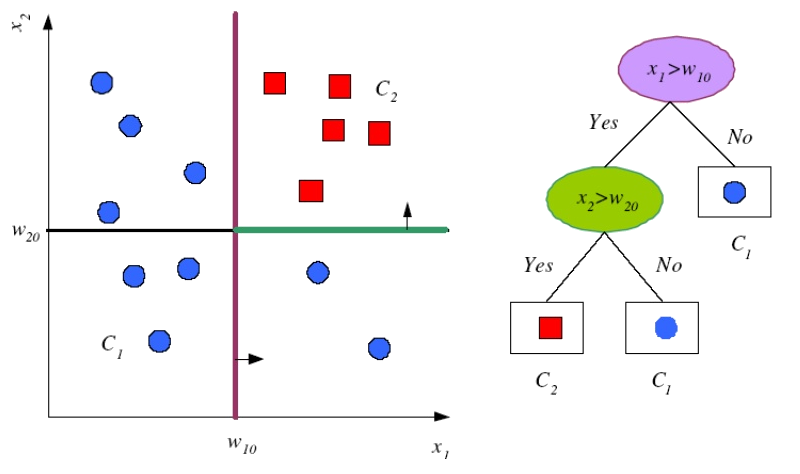
\includegraphics[width=\textwidth]{dt.png}
		\end{figure}
	\end{frame}

\end{document}
